
\chapter{Background}\label{chapter:background}

\section{The Trainbenchmark Framework}\label{section:trainbenchmark}

In the following section, we introduce Train Benchmark, a framework on which our search is based to find empirical connections between
different models and the related evaluated queries in order to estimate query evaluation time. The next few sections explain the main goal of the framework and represent the most important components in the system on which we will concentrate in the later chapters. Apart from these, we also allude some obsolete parts of the framework and emphasize their disadvantages in order to make understandable the main motivation of design decisions that resulted in some considerable modifications in the system.

\subsection{Main Concepts}

The basic idea and implementation of the Train Benchmark framework was introduced by the Fault Tolerant Systems Research Group in the Budapest
University of Technology and Economics. The implementation is written in Java programming language. Basically, Train Benchmark focuses on the performance of model validations in which the goal is to find those elements from a model that violate the well-formedness constraints. \footnote{A well-formedness constraint is defined on the model and it is considered as a definition of a particular rule belonging to the elements in the model. For example, a constraint can order the cardinality of the elements, or it can define maximum bounds for attributes, etc.} The model validations are accomplished by different databases systems, where the validation appears as a query evaluation, and the measured performance by the system is the evaluation time of the particular query. For the sake of clarity, Figure 1 represents the main steps of the framework's workflow.

The first step is the model generation and the definition of the well-formedness constraints. The Train Benchmark framework uses artificially generated graph-based models with the same domain, it and describes different constraints on them. Since the main goal is to assess model validations, a perfectly valid model generation is not advisable, thus, some fault injections are required during the generation phase, when a subset of the elements (typically 2-5\%) violates the well-formedness constraints. 

The second step is loading the model to the database systems. Subsequently, the generated model is already accessible from the database's repository, and stored in their own format. The next phase is the model validation itself, when a validation---defined in the particular database's query language---is evaluated and its result set includes those erroneous elements from the model that violate the well-formedness constraints. Thus, a model validation occurs and the required time of the query evaluation is measured as well. The validation time will play the most important indicator in the performance comparison among different databases.
 %todo insert validation pic
To summarize, the Train Benchmark framework uses artificially generated graph-based models to investigate the model validation times and thus, the performance of different database systems. In the following, we introduce the domain of the model and its typical characteristics, furthermore, we also define the scope of the framework, as represent the used databases.

\subsection{The Metamodel} \label{section:metamodel}

As we referred in \ref{section:trainbenchmark}, there were some components in the Train Benchmark framework that needed to reconstruct in order to obtain precise statistical analysis of model and query metric relationships. One of them was the original domain of the framework, the metamodel. However, (i) to understand the motivations of changing the domain entirely, (ii) to see the contrast between the two of them, and (iii) also recognize the possible virtues that we obtained by introducing a now domain, it is important to represent the original domain in this section.

At first, let define the basic related concepts.

\paragraph{Metamodel and Instance Model}

A metamodel is considered as an abstract model of another model, where the prior---the metamodel---defines the available elements and their cardinalities, additionally, it order rules, constraints on the elements which are used in the latter. Then, a concrete instance of a metamodel is called instance model which can use those elements that are defined in the metamodel, and it must also obey the specified rules and constraints, otherwise, it is considered as an invalid model which violates the constraints in the metamodel.

The domain, or the metamodel\footnote{We use the concepts of domains and metamodels as synonyms in this paper.} of Train Benchmark is depicted in Figure 2, and it is related to a railway network (here comes the name of the benchmark framework). A train route is defined by a sequence of sensors. Sensors are associated with track elements which are either segments (with a specific length) or
switches. A route follows certain switch positions which describe the required state of a switch belonging
to the route. Different route definitions can specify different states for a specific switch. Each route has
a semaphore on its entry and exit~\cite{train_ttc}.

The instance models are not related to any real life data, since the instances are generated artificially, and each cardinality of the elements originally was chosen arbitrarily. As a consequence, we cannot associate our models to real life topologies, and thus, we are not able to draw conclusions after our benchmark results in real life situations. Figure 3 shows the cardinalities of the elements, which leads to the fact that segments represent the majority of the elements.

Later, we will query the inflexibility of this metamodel, referring to some heterogeneity problems, and decide to change the domain entirely that is already appropriate for our purpose.

\subsection{Supported Formats}

The statement that the Train Benchmark framework assesses the performance of different database systems is not entirely true. Actually, the scope of the framework is extended, since we also measure various application programming interfaces (API) which are able to store the data in memory, and behave as embedded databases, furthermore, we investigate the performance of different query engines and business management tools. In order to avoid the misunderstandings and use a common expression for these systems, from now on, we reference them as \textsf{tools}.

The currently supported tools can be categorized into four different formats. These categorizations do not only mean conceptual differences, but these appear in the framework's architecture as well. The formats are the following:

\begin{itemize}
	\item SQL: This category includes the Relational Database Management Systems (RDBMS) that are based on relational models. The format was given its name after the query language of these tools that is formulated in Structured Query Language (SQL).
	\item EMF: The EMF abbreviation denotes the Eclipse Modeling Framework that facilitates the usage of model-driven development,
	as it focuses on the creation and applicability of domain models~\cite{emf}. Previously, in Section \ref{section:metamodel}, the metamodel in Figure 1 %TODO figure 1 
	was created with EMF.
	\item Graph: That tools are involved in this format which operate as graph databases and typically use the GraphML format for their primary data storage structure~\cite{graphml}.
	\item RDF: The majority of the tools are related to the Resource Description Framework (RDF). Our search highly concentrates on these systems, therefore, Section \ref{section:rdf} introduces the main concepts of RDF in details.
\end{itemize}

In the further sections, we only focus on the subset of Graph- and RDF-based tools.

\subsection{Performance Comparison and Uniformity}

After introducing the main concepts, the metamodel, and the different formats belonging to Train Benchmark, it is necessary to explain the performance comparison in more details.

Initially, clarify the meaning of performance in the case of Train Benchmark. The key concept on which the framework concentrates the most is the model validation, and thus, under the concept of performance is meant the required time of model validations. The measured validations are executed by various tools, and thus, a concrete validation time characterizes the performance of the particular tool. To summarize, the Train Benchmark framework assesses various tools and their query evaluations performance via model validations.

One important approach of the performance investigation is the scalability of the tools. In order to asses scalability, the benchmark uses instance models of growing sizes, and each model contains twice as many model elements as the previous one.

As it was already emphasized, the benchmark framework measures various tools with different supported formats which naturally indicates the diversity of the instance models. In order to prevent dissimilarities among instance models, the Train Benchmark framework constructs abstract models during the generation phase, independently on formats, and then these models are persisted to the individual acceptable formats belonging to the tools. As a result, the model generation does not depend on the specific formats, and thus, a uniform model is mapped and used by the various implementations. The most important consequence from this fact is that the performance comparison becomes possible among the tools, since they all execute the same validations on the same structured models.

Besides uniformity, it is essential to guarantee reproducibility of the instance models. In order to achieve this, we use pseudo-random\footnote{It is an algorithm for generating a sequence of random numbers, but actually it can be completely
	determined by a relatively small set of initial values, called the pseudorandom generator's seed.} generators which makes the model precisely reproducible.

\subsection{The Foundations of the Framework: Tools}

In terms of the implemented tools in the benchmark framework, it is already explained that they are categorized into four different formats. These tools are listed in Table \ref{tab:tools}. Unfortunately, we cannot afford in our research to investigate and analyze all of the currently integrated tools from the framework, hence, we chose a subset of the tools, and typically focus on the RDF-based systems. The analyzed tools on which we concentrate are marked in bold in the table.

\subsection{The Framework's Architecture}

It is important to emphasize that our goal in this paper is not entirely related to the main motivation and aim that belong to the Train Benchmark framework. We are not concerned with model validations (or transformations\footnote{Some instance model transformations are also occurred in the workflow of Train Benchmark after each validation. The goal is to investigate how the implemented tools perform after certain model modifications so that they execute the same validations and transformations again, iteratively. Since currently this area is out of our scope, we do not describe it in details.}) %todo right here in a footnote? seriously? 
, instead, we pay more attention to the first query evaluations and the precise characterization of the model. The latter option is entirely missing from the framework, since we cannot calculate metrics connected to the instance models. However, the embedded model validation components---and the integrated tools themselves---are reusable for our purpose.

Figure 4 depicts the main components are found in the benchmark framework. Based on this, it is clarified which components can be reused, and which needs to be extended or reimplemented completely for our purpose. The first considerable alteration is the \textsf{Generator} unit, which is responsible for the graph-based model generation on an abstract layer, meaning that the component operates independently on the existing formats. Which components are responsible for parsing the model to the specific format, those are the \textsf{FormatGenerator} units. Only the RDF-based component needs to be extended. The generation related modifications are described later in details.

As far as the \textsf{Validation} unit is concerned, it can be reused, independently from the fact that we do not consider model validations in our search, however, the query execution units can be utilized.

The \textsf{Publisher} component provides the measurement results and serializes them to the disk in JSON formats.

In summary, the framework's architecture provides an appropriate base to investigate the relationship among the precise characterization of a model, the composition of a particular query, and the evaluation itself.

\section{Basic Statistics} \label{section:distributions}
%todo train előtt vagy után legyenek a statos fejezetek?
In this section we present the fundamental concepts of the field of statistics. It is important to emphasize that we do not have the intention to cover most of the theorems in statistics, on the contrary, this section only introduces briefly the important concepts on which our search is based. The majority of the definitions can be found in~\cite{statistics_book}.

\subsection{Study and Experiment}

In a \textbf{designed experiment} the engineer makes purposeful changes in the controllable
variables of the system or process, observes the resulting system output data, and then
makes an inference or decision about which variables are responsible for the observed changes
in output performance. 

In an \textbf{observational study}, the engineer observes the process, disturbing it as little
as possible, and records the quantities of interest.

The main essential difference between them is that randomized experiments allow for strong claims about causality\footnote{Causation indicates that one event is the result of the occurrence of another event, which means, there is a causal relationship between the two of them.}.

\subsection{Population and Sample}

A \textbf{population} is a large set of objects of a similar nature which is of interest as a whole. On the other hand, a \textbf{sample} is a subset of objects is drawn from a population~\cite{sample1}. Another approach to define the difference between the concepts is that a population includes all of the elements from a set of data, however, a sample consists of one or more observations from the population~\cite{sample2}.

For example, the population can be human beings, and the sample is a finite subset of humankind. To be more constructive, in our case the population contains every possible measurement, and a sample includes a several of them, restricted for a particular tool's measurement results. A population can also be imaginary. 

The sample size is the number of observations in a sample and commonly denoted by \textit{n}.

In the following chapters, we will refer to samples, as we build different ones and analyze them, respectively.

\subsection{Random Variables and Distributions}

\subsubsection{Random Variables}
In statistics, a variable is as an attribute belonging to an entity, and its value can vary from one entity to another.

When a variable exhibits variability in measurements---as some deviation can be observed between the variable's values---it is considered as a random variable. Assume that $X$ represents a measurement, then the random variable's formula is
\begin{align} \label{eq:random_variable}
	X = \mu + \epsilon
\end{align} 
where $\mu$ represents a constant and $\epsilon$ is a random disturbance.

\subsubsection{Probability Distributions}The probability distribution of a random variable $X$ is a description of the probabilities
associated with the possible values of $X$. In other words, a probability distribution links each possible value that a random variable can assume with its probability of occurrence.

One differentiates the discrete and continuous distributions, when a random variable is a discrete variable, its probability distribution is called a discrete probability distribution, similarly to the continuous one.\footnote{From now on, we only use discrete probability distributions, and in every context, we refer to discrete automatically.} %todo kell ez ide? talán elvárható, hogy tudják mi a discrete és continuous%

As we will introduce in details later, the base of our model generation is strongly connected to different discrete probability distributions. The ones that will be taken into account are introduced briefly in the following paragraphs~\cite{distributions}.

\paragraph{Uniform Distribution}

A random variable $X$ has a discrete uniform distribution if each of the \textit{n} values in
its range, say, $x_1$, $x_2$, ..., $x_n$, has equal probability. Then,
\begin{align}
	f(x_i) = \frac{1}{n}
\end{align}
where $f(x_i)$ denotes the probability distribution function.

\paragraph{Pareto Distribution}

If $X$ is a random variable with a Pareto distribution\footnote{More types of Pareto distributions are distinguished, the commonly known Type I distribution is introduced.}, then the probability that $X$ is greater than some number $\sigma$, is given by
\begin{align}
	\overline{F}(x) = Pr(X>\sigma) = \Big( \frac{x}{\sigma} \Big)^{-\alpha}
\end{align}
where $\sigma$ is the scale, and $\alpha$ represents the shape parameter($x$ > $\sigma$, $\sigma$ > 0).

A similar approach is the power-law distribution which describes the probability of the random variable $X$ that---on the contrary of the Pareto distribution---is not higher, but equals to $x$. This leads to
\begin{align}
	f(x) = c\cdot x^{-\gamma}
\end{align}
where $c$ is a constant and $\gamma$ is called as the \textit{exponent} or \textit{scale factor}. Later, we will increasingly pay attention to the power-law distributions.

\paragraph{Poisson Distribution}
The Poisson distribution is characterized by the following elementary probabilities:
\begin{align}
	P(X = k) = \frac{\lambda^k}{k!}e^{-\lambda}
\end{align}
where $\lambda$ > 0 is the shape parameter and $k$ $\in$ $\mathbb{N}$.

%todo insert distributions pic%

\subsection{Related Measurements}

It is essential to introduce some measurements related to random variables and their probability distributions on which we will refer later.
\subsubsection{Mean}
The \textit{mean} or \textit{expected value} of a discrete random variable $X$, denoted as $\mu$ or $E(X)$, is
\begin{align}
	\mu = E(X) = \sum_{x} xf(x)
\end{align}
where $x$ represents the values of the random variable $X$, and $f(x)$ is the probability distribution function. A mean is a measure of the center of the probability distribution.

\subsubsection{Variance}

The \textit{variance} of $X$, denoted as $\sigma^2$ or $V(X)$, equals to the following formula:
\begin{align}
	\sigma^2 = V(X) = E(X - \mu)^2 = \sum_{x}(x - \mu)^2 f(x)
\end{align}

The variance is a measure of the dispersion, or variability in the distribution, as it represents the average of the squared differences from the mean. For example, a variance of zero indicates that all the values are identical.

\subsubsection{Standard Deviation}

The \textit{standard deviation} of the random variable $X$ is $\sigma = \sqrt{\sigma^2}$, thus, it is the square root of the variance.

\subsection{Covariance and Correlation}

\subsubsection{Covariance}
\textit{Covariance} is a measure of linear relationship between the random variables. The covariance value between two random variables $X$ and $Y$ can be expressed by
\begin{align}
	cov(X,Y) = E\big[(X - \mu_X)(Y - \mu_Y)\big]
\end{align}
where if $cov(X,Y) > 0$, then $Y$ tends to increase as $X$ increases, and if $cov(X,Y) < 0$, then $Y$ tends to decrease as $X$ increases~\cite{covariance}. A few examples are depicted in Figure 1 %todo covariance pictures from 198%
in different scenarios where---in the terms of Figure (a) and (b)---a covariance is observable between $X$ and $Y$, however in Figure (c) and (d), the covariance equals to zero.

\subsubsection{Correlation}
Similarly to covariance, a \textit{correlation} describes the strength of the relationship between variables. A type of correlation, the Pearson product-moment correlation coefficient is formulated as
\begin{align}
	\rho_{XY} = \frac{cov(X, Y)}{\sigma_X\sigma_Y}
\end{align}
where $ -1 \leq \rho_{XY} \leq 1$, and 1 indicates a total positive linear relationship between $X$ and $Y$, -1 means negative linearity, finally, 0 is interpreted as a correlation does not exist between the variables.

\subsection{Regression Analysis}

\textit{Regression analysis} is a statistical technique for exploring the relationship between two or more variables. A regression model can be considered as an equation that relates a random variable $Y$ to a function of a variable $x$, and a constant $\beta$. In formally, a regression model is defined as
\begin{align} \label{eq:linear_regression}
	Y = \beta_0 + \beta_1x + \epsilon
\end{align}
where $Y$ is the dependent or response variable, $x$ is called as an independent variable or predictor, and $\beta_0$, $\beta_1$ are the regression coefficients, the intercept and the slope, respectively. Finally, $\epsilon$ is a random error. More precisely, Equation \ref{eq:linear_regression} is called a \textit{linear regression model}, since it uses one independent variable to predict the outcome of $Y$.

A multiple linear regression model considers $k$ independent variables, and the equation is extended as the following
\begin{align}
	Y = \beta_0 + \beta_1x_1 + \beta_2x_2 + \dots + \beta_kx_k + \epsilon
\end{align}

\section{Graph Theory}

In the following sections we introduce the most important graph metrics and network topologies on which we concentrate in our work. We assume that the reader is already familiar with the basics concepts of graph theory, including directed graph, connectivity, complete graph, adjacent nodes and
degrees of vertices.
%todo fix these metrics 
\subsection{Metrics}

\subsubsection{Degree Distribution}

The fluctuation among the degrees of the nodes is characterized by a distribution function $P(k)$ which shows the probability that a randomly selected node's degree is equal to $k$. $P(k)$ is called as the degree distribution.

\subsubsection{Clustering Coefficient}

The $C_n$ clustering coefficient of an $n$ node is equal to the proportion of connections among those vertices that are adjacent to $i$ divided by the maximum number of connections that can be drawn between them. Formally written, in undirected graphs $C_n = \frac{2\cdot e_n}{k_n\cdot(k_n-1) }$, where $k_n$ is the number of neighbors of $n$ and $e_n$ is the number of connected pairs between all neighbors of $n$ (~\cite{clustering_formula}). As a result, the clustering coefficient is always quantified between 0 and 1.

An example is showed in Figure \ref{fig:clustering}. In this case, the clustering coefficient of \textsf{A} is $C_A = \frac{2}{6}$, since it has three neighbors, so $k_A = 3$, and only one connection occurs among its adjacent nodes---between \textsf{B} and \textsf{C}---indicates that $e_A = 1$.
\begin{figure}[!ht]
	\centering
	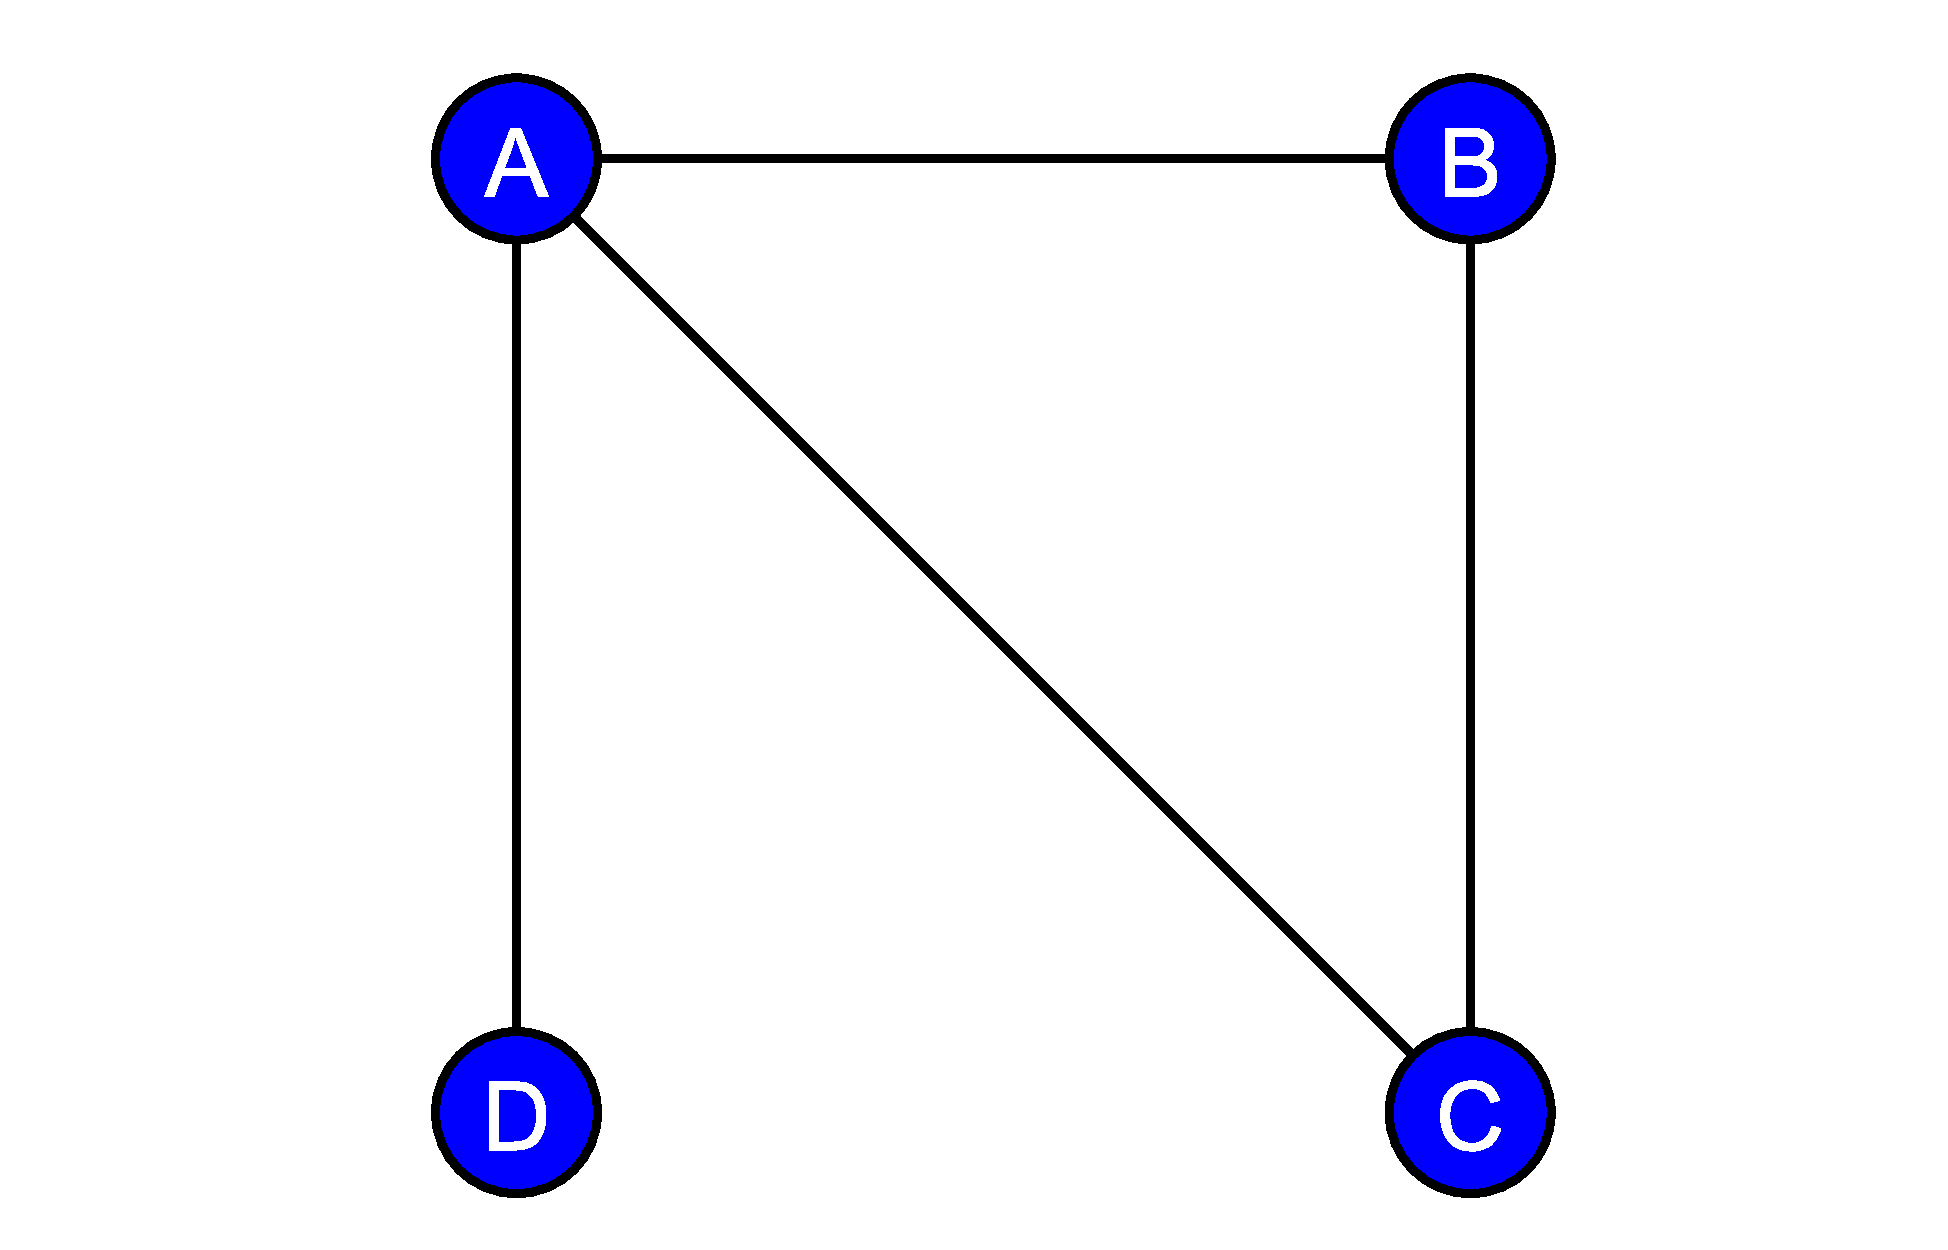
\includegraphics[width=60mm, keepaspectratio]{figures/clustering.pdf}
	\caption{An example graph for illustrating the calculation of clustering coefficient.}
	\label{fig:clustering}
\end{figure}

\subsubsection{Betweenness Centrality}

The betweenness centrality of an $n$ node is quantified by the number of shortest paths that include $n$ as an intermediate node, divided by the total number of shortest paths. Consequently, this metric is mapped between 0 and 1.

\subsection{Network Topologies} \label{sec:topologies}

\subsubsection{Random Graph}

\subsubsection{Small-World Model of Watts-Strogatz}

\subsubsection{Scale-Free Model of Barabási and Albert}

\subsubsection{Hierarchical Network}
\section{Resource Description Framework: RDF} \label{section:rdf}

